\chapter{AI as the Infrastructure of Modulation}
\glsresetall

\epigraph{[...] descending into the hidden abode of production means something else in the digital age. It means that we must also descend into the somewhat immaterial technology of modern-day computing, and examine the formal qualities of the machines that constitute the factory loom and industrial Colossus of our age. The factory was modernity’s site of production. The “non-place” of Empire refuses such an easy localization. For Empire, we must descend instead into the distributed networks, the programming languages, the computer protocols, and other digital technologies that have transformed twenty-first-century production into a vital mass of immaterial flows and instantaneoustransactions. Indeed, we must read the never ending stream of computer code as we read any text (the former having yet to achieve recognition as a “natural language”), decoding its structure of control as we would a film or novel.}{\cite[82]{galloway2001}}


\greensquare

Contemporary \gls{ai}, and particularly \gls{genai} and \glspl{llm} operate through architectures that capture and recombine traces of language while parsing the collection of human knowledge. If control societies are defined by infrastructures that capture, modulate, and recombine traces of life, contemporary \gls{ai} embodies this logic in its technical architecture. To understand how these systems participate in the production of subjectivity, we must first trace the historical and technical evolution of AI, from symbolic reasoning to statistical modeling and self-attentive transformers.

The current chapter provides the technical foundation for the subsequent political analysis of generative AI. To properly understand the potentially institutional role of \gls{genai} models, and \glspl{llm} in particular it is necessary to first trace their historical development, underlying architectures, and operational logics. While this section remains on a primarily technical level, it also gestures towards the epistemological and political stakes that will be discussed later.
%The chapter proceeds chronologically and conceptually.
It begins by outlining the historical trajectory of artificial intelligence research, distinguishing between the early, symbolic paradigm (\gls{symai}) and the contemporary, statistical approaches that characterize \gls{dl}  and \gls{genai} models. This includes an explanation of neural networks, self-supervised learning, and the rise of transformer architectures as the technical backbone of modern \glspl{llm}.

Beyond mere description, this technical overview serves a strategic purpose: it demonstrates how AI, even at the level of architecture, already embeds specific logics of inference, representation, and control. These are not neutral technical details, but the material conditions that enable AI systems to operate as infrastructures of knowledge production, decision-making, and ultimately, governance. The subsequent sections therefore provide both the necessary technical background and the conceptual scaffolding for the analysis of generative AI as a distributed, non-symbolic institution of power.




\marginnote{
	\begin{orangebox}
		This part can be a good addition to the "state of art"

		\begin{itemize}
			\item \cite{montanari2025} is a good source for a brief techno-political
			      history and genealogy of llms
			\item Also here
			      https://www.technologyreview.com/2024/07/10/1094475/what-is-artificial-intelligence-ai-definitive-guide/
			      and here \cite{pasquinelli2023}
		\end{itemize}
	\end{orangebox}
}

\section{From Symbolic Rules to Statistical Modulation: A Brief History of \gls{ai}  and \gls{nlp} }

\greensquare
\Gls{nlp} is an area that lies at the intersection of linguistics, computer science, and AI, aiming to create computational systems that can interpret and handle human language data. Considering that, in some respects, the cognitive performance of an individual human is hardly superior to that of other primates \parencite[127]{manning2022a}, it is hardly surprising that breakthroughs in \gls{ai} have been driven by \gls{nlp}. Language, more than individual brainpower, constitutes the machinery through which human intelligence scales, distributes, and accumulates collectively \parencite[127]{manning2022a}, and has been the ground most of the breakthroughs in \gls{ai} development, especially, in the recent years (see \cite[22ff]{bommasani2022a} for a detailed analysis of the history of \gls{ai} and language).

\marginnote{\textbf{TODO}: Title
	\begin{todolist}
		\item A little more articulation is needed around here.

	\end{todolist}
}


\greensquare
Artificial intelligence emerged in the mid-20\textsuperscript{th} century, grounded in the formal logics of symbolic representation. The foundational paradigm, now referred to as \gls{symai} or \gls{gofai} , conceived intelligence as a matter of symbolic reasoning over explicitly encoded rules. The early paradigm treated intelligence as a computational process operating over discrete symbols according to explicitly programmed rules. AI systems under this logic were built to emulate deductive reasoning and problem-solving. The assumption was clear: if the world could be faithfully translated into a logical schema, machines could infer, deduce, and act rationally (see \cite[183]{eloff2021}).

\greensquare
\textcite{manning2022a} defines the \textbf{first era} between 1950 to 1969 as a development process under the immense lack of
the knowledge about structure of human language or \gls{ml} and \gls{ai}. The
1956 Dartmouth Conference institutionalized the ambitions by defining AI as
``the science and engineering of making intelligent machines''
\parencite[195]{montanari2025}. Early research during this period was primarily focused on narrow, rule-based systems, particularly word-level translation lookups and simple mechanisms to handle inflectional forms and word order \parencite[128]{manning2022a}.
In parallel, Alan Turing made substantial contributions by introducing the famous "Turing Test" (or "Imitation Game"), designed to evaluate a machine's ability to imitate human intelligence and rationality, along with the foundational concept of a universal machine (see \cite[196]{montanari2025}). As Cognitive Robotics Prof. Murray Shanahan and Meta's Chief AI scientist Yann LeCun emphasize, the \textit{Turing Test} is an inadequate benchmark for assessing modern \gls{ai} models \parencite[]{lexfridman2024, googledeepmind2025}, but Turing's ideas nonetheless contributed to the conceptual foundation of the \textit{prompt-based conversational machine} \parencite[196]{montanari2025}. Aligned with Turing's perspective, the underlying notion in the early imaginary of a future \gls{ai} was simple; if a machine could convincingly imitate a human in conversation, it was considered intelligent.

\greensquare
Relying on handcrafted rule sets included implicit definitions of the features regarding the object of interest; to recognise patterns the digit six in an image for instance, one might encode the features "a closed loop at the bottom" and "a curve rising to the right". Such symbolic heuristics were sufficient so long as the data was clean and the context unambiguous. In the \textbf{second era} of \gls{ai} development, spanning roughly 1970 to 1992, these approaches were extended to more complex domains, most notably natural language. By attempting to formalize aspects of linguistic structure and meaning, researchers pushed the boundaries of rule-based systems. While these models demonstrated greater sophistication in handling linguistic patterns, they still relied on explicitly encoded knowledge and remained limited by the inherent rigidity of symbolic architectures \parencite[129]{manning2022a}. Yet, these systems could not generalize beyond predefined rules. When confronted with noise or shifting contexts, their logic collapsed. The result was a period of stagnation and disillusionment now remembered as the "AI Winters" between 1970 - 1980 \parencite[183]{eloff2021}.
\sidenote{\textbf{TODO:} A more nuanced explanation regarding the transformation is needed,
	e.g. \cite{pasquinelli2023}.}


\greensquare
But real-world ambiguity proved hostile to symbolic systems. As \gls{symai} attempted to scale into more complex domains like vision or language, it revealed its brittleness \parencite[183--184]{eloff2021}. Philosophers of phenomenology were early critics of this paradigm following Hubert Dreyfus' (\cite*{dreyfus2009}\sidenote{Originally published in 1972.}) earlier work where he argued that human intelligence was not symbolic, but embodied, situated, and fundamentally non-representational. Despite such critiques, \gls{symai} dominated the earlier decades of research in \gls{ai} fields. This rationalist framework aligned with early cognitive science’s attempts to model the mind as a rule-based machine of symbolic representation (see \cite[194--197]{montanari2025}). \gls{dg} were also one of the ciritiques, the hierarchically structured learning and the projection of a central pattern was clearly not working well:

\begin{quote}
	This is evident in current problems in information science and computer science, which still cling to the oldest modes of thought in that they grant all power to a memory or central organ. Pierre Rosenstiehl and Jean Petitot, in a fine article denouncing "the imagery of command trees" (centered systems or hierarchical structures), note that "accepting the primacy of hierarchical structures amounts to giving arborescent structures privileged status.... The arborescent form admits of topological explanation.... In a hierarchical system, an individual has only one active neighbor, his or her hierarchical superior.... The channels of transmission are preestablished: the arborescent system preexists the individual, who is integrated into it at an allotted place" (signifiance and subjectification).

	— \cite[16]{deleuze1987}
\end{quote}

\Gls{dg}’s critique of early AI approaches centred on their rejection of hierarchical and centralised models which constitute one of the main pillars of their project. Their affirmative alternative was grounded in a connectionist and non-hierarchical understanding of thought, formalised through the concept of the \textit{rhizome} \parencite[3ff.]{deleuze1987} as in opposition to \textit{tree} structures. While their critique targeted the symbolic, rule-based systems of their time, it is striking how closely their vision anticipated the architectural principles underpinning contemporary \gls{ai} on a general level, particularly in its distributed, associative, and layered formations
\sidenote{Arguably, also regarding non-hierarchical functioning of the \glspl{nn};
	however, it is still a matter of discussion, if the \gls{genai} model
	architectures deploy a contuinuous subordination between different patterns and
	distributions. See the following sections for further articulations.}
. Nonetheless, the technological trajectory toward such architectures would take decades to materialise, revealing the prescient force of their philosophical intervention.

\greensquare
The \textbf{third era}, from roughly 1993 to 2012, was signified with the beginning of
the abundance any novel \gls{ai} innovation lacked the most, \emph{the data}. As the internet boom suddenly introduced a massive digital corpora, researchers shifted toward statistical learning, leading to the rise of data-driven \gls{nlp}. This shift replaced hand-coded rules with empirical models trained on annotated examples \parencite{maas2023}; models could now generalize from data rather than deduce from explicitly defined axioms. Initially, the dominant approach centered on relatively simple statistical techniques applied to modest amounts of text, often in the low tens of millions of words. Researchers extracted linguistic facts from these corpora, identifying regularities such as common collocations or syntactic structures. Yet, early attempts to model language understanding through these means remained limited in their ability to capture deeper semantic or contextual knowledge (see \cite[129]{manning2022a}). For instance, early statistical models revealed that certain types of words tended to appear together, names of places often occurred alongside personal references, while more abstract terms exhibited distinctive distributional patterns. However, such surface-level regularities provided only limited insight into the deeper structures of language. As it became evident that simple frequency-based methods were insufficient for capturing the complexity of linguistic meaning, the focus shifted toward building annotated linguistic resources, such as syntactic treebanks, lexical databases, and labeled datasets for named entity recognition. These resources formed the foundation for more reliable, supervised learning approaches (see \cite[129]{manning2022a}). Onwards, the general purpose \gls{ai} development continued with ups and downs in activity, with a couple of earlier succesful neural network based aproaches like Mulloch-Pits. Among the early milestones was ELIZA, a rule-based program that mimicked a psychotherapist by matching keywords to scripted responses. Despite its simplicity, ELIZA gave the illusion of understanding and demonstrated the potential of machine conversation; though its developer emphasized it was merely parodic \parencite{toloka2023}. Still, it signalled the beginning of natural language interaction with machines, laying groundwork that statistical and later neural methods would build upon. Up until around 1997 where much more advanced models like Deep Blue operating on more sophisticated architectures like the early attempts on \glspl{dnn} were developed \parencite[197]{montanari2025}, but the main meta of the \gls{ai} development was highly dependent on labeled data, and \gls{sl}.

\marginnote{\textbf{TODO}: Title
	\begin{todolist}
		\item Add the BA history info here
		\item Explain \gls{sl}

	\end{todolist}
}

Although, the real transformation originally began in the early 2000s, the first significant fruits of the new direction dropped around 2013, which marks the \textbf{4. and current era} in \gls{ai} development \parencite[129]{manning2022a}. Pushes through the ability to process more and more data allowed a new paradigm to emerge, rooted in \glspl{nn} inspired by the architecture of the brain, \emph{connectionism} became the new meta of further advancements. These systems, now more broadly applied and clearly defined as \glspl{dnn}, learned not by logic but by adjusting distributed weightings across layered networks, which became the foundation for contemporary \gls{ml} and \gls{dl} systems. Exponential advances in computation enabled these networks to scale \parencite[184]{eloff2021} and finally also pushed towards an \gls{ul}\sidenote{Should this one have its own section?}  methodologies, whereas the models were geared towards to recognise patterns in the data without being explicitly told which features of the data were pointing to what. For instance, while early augmentational models were trying to distinct between cat and dog photos by looking at photos labeled by humans and other processes as either as \textit{dogs} or \textit{cats}, \gls{ul} models are looking at a data collection of unlabeled photos and try to find patterns in them which makes both parties distinct through specific characteristics, in other words, towards finding out about the substance of \textit{dogness} and \textit{catness}. On the \gls{nlp} fronts, linguistic units such as words or sentences came to be represented as vectors in high-dimensional vector spaces. Semantic and syntactic relationships were modeled not through rule-based analysis and pre-defined categories, but through the spatial proximity of these vectors \parencite[129]{manning2022a}. \Gls{dl} allowed to parse distant context, as well as, processing the words meaningwise close to each other thanks to this generalised vector space approach optimised with more and more textual data (see \cite[129]{manning2022a}). This approach turned out to be far more effective than earlier attempts at formalizing linguistic meaning. Instead of hand-coding grammatical rules or manually annotating small corpora, models could now process large textual datasets and infer structure statistically. \Gls{dl} enabled systems to capture long-range dependencies in context and identify meaning-level relationships through learned representations optimized across massive datasets. Crucially, this reduced the need for manual labeling, as \gls{ul} techniques became dominant.

\marginnote{\textbf{TODO}: Title
	\begin{todolist}
		\item Better citations needed in this part
		\item We could also mention the Saussarean assumption here.
		\item Refer to Figure 1 in \cite{manning2022a}

	\end{todolist}
}

One of the most significant turning points was around 2018 with the succesful implementation of \gls{ssl} approach. \Gls{ssl} constitutes a special case of the \gls{ul} which not only makes the models identify underlying structures in the data but also enables them to create their own training exercises through the prediction challenges they are subjected to \parencite[129]{manning2022a}. This includes masking specific words in the text to try to predict correct or most fitting \glspl{token}, or try to guess the next word in an abruptly cut text, \gls{ssl} models learn by predicting missing elements from within the input itself. This method allowed models to learn linguistic regularities from massive unlabeled corpora, and it gave rise to pre-trained \glspl{genai} \parencite{maas2023}. The architecture that enabled this leap was the \textit{transformer architecture}. Its core mechanism, self-attention, computes weighted dependencies between all tokens in a sequence, allowing the model to capture long-range relations independent of word order. This innovation enabled massive parallelization and scalability \parencite{maas2023}. Availability of vast data and the unique novelty of transformer architecture that was powered by a huge amount of reinforcement capability through repetition has been crucial operating on \gls{ssl} methodology to parse and accumulate huge amounts of unlabeled human language data. The transformer architecture is fundamental for the meaning-making capability of the \gls{genai} models, the following sections is therefore dedicated to focus on this specific innovation.


\sidenote{\textbf{TODO:} There needs to be a section about supervised ->
	unsupervised learning since unsupervised learning marks the rise of neoplatonic
	esoterism.}


\marginnote{\textbf{TODO}: Title
	\begin{todolist}
		\item Update the following paragraph

	\end{todolist}
}



\begin{orangebox}


	A subcategory of the \gls{genai}, \glspl{llm} such as GPT-3 and GPT-4 are not task-specific in the traditional sense. Rather than being fine-tuned for each use case, they rely on ``few-shot prompting'': given a small set of examples at inference time, they condition their outputs without internal weight updates. Their knowledge is distributed across billions, sometimes trillions, of parameters trained to minimize prediction error. The shift from \gls{symai} to deep, generative architectures does not merely mark a technical transition. It signals a deeper epistemological break. \Glspl{llm} do not ``understand'' language in any classical sense, they generate statistically likely continuations. Meaning is no longer rule-based; it is computed as vector proximity in high-dimensional space \parencite[199]{montanari2025}. These networks are opaque, their training data culturally saturated, and their outputs probabilistic \parencite[186]{eloff2021}. They do not interpret, they modulate. Rather than representing knowledge, they operationalize its prediction. In doing so, they establish a new infrastructure for language: distributed, non-symbolic, and non-transparent.

	This transformation, from formal logic to differential modulation, sets the stage for understanding \gls{genai} not just as a technical system but as an institutional form---a mechanism of governance, sense-making, and subjectivation in contemporary control societies.

\end{orangebox}

\marginnote{\textbf{TODO}: Title
	\begin{todolist}
		\item Advance on this and introduce a smooth transition


		\item use \cite{toloka2023} Development of generative AI section to
		advance further

	\end{todolist}
}



%\section{From Rule-Based NLP to Generative Modeling}
%
%A historical typology of \gls{nlp} distinguishes four successive eras \parencite{maas2023}. The first (1950–1969) centered on word-level translation using rudimentary rule-based systems, constrained by limited linguistic and computational knowledge. The second (1970–1992) introduced more refined, hand-crafted rule systems that distinguished between declarative grammar rules and procedural language use. In the third era (1993–2012), the availability of digital text enabled supervised machine learning approaches to NLP, using annotated corpora to train statistical models that could generalize from labeled examples.
%
%\sidenote{\textbf{TODO:} Introduce better citations}
%
%The fourth era (2013–present) introduced deep learning and self-supervised training. This shift marked a decisive move away from symbolic encoding toward data-driven pattern recognition. \glspl{llm} learn by predicting masked or subsequent words in vast unlabeled text corpora. These self-supervised tasks enable the model to internalize complex linguistic regularities without human annotation, forming layered, distributed representations across billions of parameters \parencite{maas2023}.
%
%The Transformer architecture—now foundational to \glspl{llm}—relies on the mechanism of \gls{selfattention}, which computes weighted dependencies between all tokens in a sequence, allowing the model to integrate long-range context independently of position. This design enables massive parallelization and has proven essential to scaling up model complexity and generalization capabilities \parencite{maas2023}. Where early \glspl{ann} required \gls{finetuning} for specific tasks, modern \glspl{llm} operate through \gls{prompting}: conditioned on examples at inference time, they adapt behavior without internal parameter updates.
%
%This transformation marks a fundamental departure from rule-based reasoning to statistical sequence modeling. The model no longer ``understands'' language in a semantic sense but estimates the most likely continuation based on learned distributional patterns. \glspl{llm} thus operate as probabilistic engines of language generation—trained not to reason symbolically but to modulate plausible outputs within vast representational spaces \parencite{maas2023}.

%\section{Rise of Non-Symbolic AI and the Return of Connectionism}
%
%This mode of operation included the explicit definition of features to be interpreted. For example, to identify the number six, one might encode rules such as ``a closed loop at the bottom'' and ``a rising curve to the right.'' These heuristics were treated as sufficient for inference, provided the environment was clean, structured, and semantically unambiguous. Such assumptions persist in popular imaginaries, where intelligence is imagined as a disembodied capacity for symbolic manipulation. However, \gls{symai} struggled with tasks outside rule-bound domains and failed to process real-world complexity \parencite[183--184]{eloff2021}. Phenomenological critiques argued that intelligence is embodied, situated, and non-representational, challenging the epistemology of symbolic computation \parencite[183]{eloff2021}. As \textcite{montanari2025} shows, \gls{symai} remained an artifact of rationalist heritage, aiming to formalise human thought as rule-bound behaviour in tree-like hierarchies.
%
%Despite such critiques, \gls{symai} dominated early AI. The Dartmouth Conference in 1956, often cited as AI's point of origin, defined the field as the ``science and engineering of making intelligent machines,'' placing symbolic manipulation at the center of its epistemic frame \parencite[195]{montanari2025}. Early systems like Newell and Simon's Logic Theorist and expert systems in the 1970s operationalized this vision. But symbolic systems proved brittle in the face of ambiguity and noise. These limitations catalyzed the ``AI Winters'' of the 1970s and 1980s \parencite[183]{eloff2021}.
%
%The early 2000s marked the resurgence of \gls{ai} via connectionism. This paradigm, inspired by biological neural networks, abandoned symbolic representations in favor of statistical learning. Connectionist systems learn not by encoding logic but by optimizing distributed weights across layered artificial neurons. This turn was enabled by exponential growth in computational resources and data availability \parencite[184]{eloff2021}.
%
%Modern machine learning, particularly in deep learning systems, replaces symbolic reasoning with correlation. Input data is propagated through multiple hidden layers and transformed via activation functions. Training adjusts internal weights through \gls{backpropagation} and \gls{gradientdescent}, generating predictions that minimize statistical error rather than representational mismatch.
%
%This shift is not merely technical but epistemological. The internal layers of a \gls{dnn} do not correspond to interpretable features but encode a ``dramatization'' of statistical differentials \parencite[186]{eloff2021}. Pattern recognition is governed by statistical proximity, not meaning; learning is not semantic but topological and differential.
%
%\textcite{montanari2025} describes this shift as a ``renaissance of distributionalism,'' where meaning is no longer tied to syntactic rules but computed as vector proximity in high-dimensional space. Models such as Word2Vec, GloVe, BERT, and GPT encode semantics via contextual patterning. This enables inference, generation, and classification by mapping tokens across distributed embedding spaces \parencite[199]{montanari2025}.
%
%The implications are far-reaching. Deep learning architectures now underlie not only \glspl{llm} but also \glspl{gan}, recommendation engines, and real-time translation systems. These architectures enact new modes of subjectivation: they classify, filter, predict, and generate—without explaining. Their opacity, termed the ``black box problem,'' has given rise to the field of \gls{explainableai}, especially in response to bias and injustice in training data \parencite[186]{eloff2021}.
%
%Thus, contemporary \gls{ai} no longer aims to simulate reasoning but to model correlations. It is a statistical, opaque infrastructure—a topology of differential learning. If \gls{symai} sought to represent the world through logic, modern \gls{nonsymai} approximates it through modulation. This sets the stage for the next chapter: generative architectures as institutions of epistemic control.
%\hline
%
%A historical typology of Natural Language Processing (NLP) distinguishes four successive eras \parencite{maas2023}. The first (1950–1969) centered on word-level translation using rudimentary rule-based systems, constrained by limited linguistic and computational knowledge. The second (1970–1992) introduced more refined, hand-crafted rule systems that distinguished between declarative grammar rules and procedural language use. In the third era (1993–2012), the availability of digital text enabled supervised machine learning approaches to NLP, using annotated corpora to train statistical models that could generalize from labeled examples.
%
%The fourth era (2013–present) introduced deep learning and self-supervised training. This shift marked a decisive move away from symbolic encoding toward data-driven pattern recognition. Large Language Models (LLMs) learn by predicting masked or subsequent words in vast unlabeled text corpora. These self-supervised tasks enable the model to internalize complex linguistic regularities without human annotation, forming layered, distributed representations across billions of parameters \parencite{maas2023}.
%
%The Transformer architecture—now foundational to LLMs—relies on the mechanism of self-attention, which computes weighted dependencies between all tokens in a sequence, allowing the model to integrate long-range context independently of position. This design enables massive parallelization and has proven essential to scaling up model complexity and generalization capabilities \parencite{maas2023}. Where early neural networks required fine-tuning for specific tasks, modern LLMs operate through few-shot prompting: conditioned on examples at inference time, they adapt behavior without internal parameter updates.
%
%This shift in architecture and training method marks a departure from rule-governed systems to statistical sequence modeling. The model no longer “understands” language in a semantic sense but estimates the most likely continuation based on learned distributional patterns. In this new configuration, LLMs function as probabilistic engines of language generation—trained not to reason symbolically but to modulate plausible outputs within vast representational spaces \parencite{maas2023}.
%\section{Rise of the non-symbolic AI and the return of connectivism}
%
%Artificial intelligence emerged as a research domain in the mid-20th century, rooted in the formal logics of symbolic representation. This early paradigm, retrospectively labelled \gls{gofai} or \gls{symai}  , treated intelligence as a computational process operating over discrete symbols according to explicitly programmed rules. AI systems under this logic were built to emulate deductive reasoning and problem-solving: if the world could be encoded in a set of symbolic propositions, intelligent behavior could be generated by manipulating those propositions through logic (see \cite[183]{eloff2021}).
%
%This mode of operation included the explicit definitions of the features to be
%interpreted, for example, in the case of hand written number recognition to identify the number six, one might encode rules such as ``a closed loop at the bottom'' and ``a rising curve to the right.'' These symbolic heuristics were treated as sufficient for inference, provided the environment was clean, structured, and semantically unambiguous. Such assumptions persist in popular understandings of AI, where intelligence is imagined as a disembodied capacity for logic and symbolic manipulation . However, symbolic AI struggled with anything beyond the environments where rules and the goals can be explicitly defined and has never been remotely capable of processing real-world complexity (see \cite[183-184]{eloff2021}). Philosophers of phenomenology \sidenote{For example \cite{dreyfus2009}.}  challenged the underlying epistemology of \gls{symai}  early on, drawing on phenomenological aspects to argue that human intelligence is irreducibly embodied, situated, and non-representational \parencite[183]{eloff2021}. \Gls{symai} stayed as one of the remnants of the rationalist heritage of early cognitive science, aiming to formalise human thought as rule-bound behaviour  \parencite[194--197]{montanari2025} and tree-like hierarchical operation.
%
%
%Despite these critiques, symbolic AI dominated the early decades of the field. The Dartmouth Conference in 1956, widely regarded as AI's founding moment, introduced intelligence as the ``science and engineering of making intelligent machines,'' laying the groundwork for symbolic manipulation as AI’s epistemic foundation \parencite[195]{montanari2025}. Systems such as Newell and Simon's Logic Theorist and later expert systems in the 1970s were emblematic of this formal, logic-driven approach. However, symbolic systems proved fragile in the face of noisy, context-rich input and failed to generalize effectively. These limitations contributed to the ``AI Winters'' of the 1970s and 1980s—periods of reduced funding and diminished confidence in the field \parencite[183]{eloff2021}.
%
%The early 2000s marked the resurgence of AI via an alternative path: connectionism. This paradigm, inspired by biological neural networks, eschewed symbolic representations in favor of statistical learning. Connectionist systems learn not by encoding logic, but by optimizing distributed weightings across layers of artificial neurons. This transition was made possible by exponential increases in computational power and data availability, which allowed deeper architectures to emerge and scale \parencite[184]{eloff2021}.
%
%Modern machine learning, particularly in its deep learning form, replaces symbolic reasoning with correlation. In an artificial neural network (ANN), input data is transformed through multiple interstitial layers into output predictions via nonlinear activation functions. In training, systems such as deep convolutional networks adjust their internal weightings by minimizing error through backpropagation and gradient descent—procedures that resemble a differential field of local adjustments rather than a global model of truth.
%
%As Eloff emphasizes, this is not just a change in method but in epistemology. The internal layers of an ANN do not resemble human-understandable features but are ``dramatisations'' of intensive differences that function without semantic transparency \parencite[186]{eloff2021}. Recognition is not governed by meaning but by statistical proximity, and optimization does not follow interpretation but numerical minimization.
%
%Montanari traces this statistical turn to a broader ``renaissance of distributionalism,'' where meaning is computed via vector space proximity, not logic. Language models like Word2Vec, GloVe, BERT, and GPT operationalize this shift by learning relationships between tokens in high-dimensional space, enabling generation and inference based on contextual patterning rather than syntactic rules \parencite[199]{montanari2025}.
%
%The implications are vast. Deep learning systems now underlie generative adversarial networks (GANs), language models, recommendation systems, and more. These architectures do not merely automate tasks; they enact new modes of subjectivation. As Eloff notes, their inner workings are opaque, their outputs probabilistic, and their training datasets culturally saturated. While they may outperform symbolic systems on tasks like image or speech recognition, they are not explainable in classical terms. This opacity, termed the ``black box problem,'' has generated calls for explainable AI, especially in light of social bias and algorithmic injustice \parencite[186]{eloff2021}.
%
%Thus, contemporary AI no longer resembles the ideal of a rational decision-maker. It is a distributed, statistical, opaque infrastructure—an algorithmic topology of differential learning. Where symbolic AI aimed to represent the world, connectionist AI aims to approximate it—less an episteme than a diagram, less a logic than a modulation. This shift sets the stage for the next chapter: the institutional implications of generative architectures.
%
%
%
%
%\hline
%\section{\acrfull{symai}}
%
%\marginnote{
%
%	\begin{orangebox}
%		This part is where you explain the whole ordeal with the BA. Old fashioned AI,
%		how it related, what it achieved and lacked
%	\end{orangebox}
%}
%
%%WARNING:MAC
%Artificial intelligence today functions as a silent infrastructure within systems of algorithmic control, embedded across platforms that shape how we search, stream, invest, and even predict criminal activity. Public imaginaries often depict AI as a kind of elevated intellect, a rational mind crafted from intricate code and formal logic, capable of solving problems through internal representations of the world. Within this vision, intelligence appears as a matter of deduction: to identify the number six, one would encode a closed bottom loop and a rising curve, operationalising recognition as the execution of symbolic (albeit self-formed by the model) rules.
%%TODO: Use your example form mathematics?
%This logic-based approach, once dominant under the banner of ‘Good Old-Fashioned AI’ (GOFAI), still echoes in certain technical domains. However, its brittleness in the face of real-world ambiguity—where data is messy, contexts shift, and meaning resists neat classification—has long rendered it inadequate. Philosophers like Hubert Dreyfus challenged this model early on, arguing that intelligence cannot be confined to syntactic manipulation, especially when embodied perception and lived experience play central roles. As such critiques mounted and expectations deflated, AI research passed through periods of dormancy (known as “AI winters”) where optimism collapsed under the weight of its own abstraction (see \cite[183]{eloff2021}).


%\section{Non-symbolic AI}
%
%Since the early 2000s, AI has undergone a dramatic revival—not as a sudden reappearance, but as a reintensification of a trajectory that never fully dissipated. At the core of this renewed momentum lies the exponential growth in computational capacity, which has reinvigorated a paradigm once sidelined: connectionism. This approach, inspired by the structure and functioning of biological neural systems, had attracted early attention in AI’s formative years. However, its practical application was curtailed by the hardware constraints of the time. What was once set aside due to technological insufficiency has now resurfaced, empowered by the capacities of modern parallel processing and data availability (see \cite[183-184]{eloff2021}). This re-initialised course was the catalysor of the development of \glspl{ann}.
%%TODO: TUrn to @eloff2021 for ANN definition
%
%
%
%
%
%\epigraph{A computer would deserve to be called intelligent if it could deceive a human into believing that it was human.}{\textcite{turing1950}}
%
%Although it is mainly discussed in a linguistic and cognitive context, \gls{ai} connects itself to some broader themes \parencite[194]{montanari2025}. The term \gls{ai} was first coined in the Dartmouth Conference as an interdisciplinary field organized by John McCarthy, Marvin Minsky, Nathaniel Rochester, and Claude Shannon at Dartmouth College; this as McCarthy stated "the science and engineering of making intelligent machines" beginning with the early 1950s was entangled with the development of field cognitive science \parencite[195-196]{montanari2025}.
%
%In \gls{AI}s early years of development, Alan Turing made substantial contributions by introducing the famous "Turing Test" (or "the imitation game") that evaluates a machine's capability of imitating intelligence and rationality of a human along with the concept of a universal machine (see \cite[196]{montanari2025}). Although, as the chief scientist leading Meta's \gls{ai} development Yann LeCun notes that the Turing Test a bad test to evaluate any kind of \gls{ai} model \parencite[]{lexfridman2024}, Turing's contributions have played its role in the conceptualisation of a "prompt"-based "conversational machine" \parencite[196]{montanari2025}. This idea was mainly framed as if a machine could convince another human to being a human, it was conceived as intelligent. Onwards, the general purpose \gls{ai} development continued with ups and downs in activity, with a couple of earlier succesful neural network based aproaches like Mulloch-Pits, ELIZA program, up until around 1997 where much more advanced models like Deep Blue operating on more sophisticated architectures like \glspl{dnn} were developed \parencite[197]{montanari2025} .

\section{Algorithmic Governance of Information before \Gls{genai} }

\begin{quote}
	Thus far, we have determined that whereas the individual and disciplinary power seem to be cast in the same mold – the former being the product of the latter – the digital subject of the control society 2.0 appears to be an active subject able to make decisions – which in turn feeds the algorithms.

	— \cite[19]{Krasmann2017}
\end{quote}


Following the historical development of the \gls{ai} models is an algorithmic
journey with a quite equivalent destination thinking about the definition of
the control society. As Deleuze expected computational systems turn into, the
use of the early \gls{nn} based \gls{ai} models was indeed focusing on the
profiling and behaviour anticipation. Before the emergence of \gls{genai}, early models emerged in search engines, social media ranking algorithms, and recommendation services, which were primarily designed for \textbf{profiling and relevance association}(see \cite[26-30]{demir2019}). Their core logic followed a recurrent loop:

\begin{enumerate}
	\item massive data collection from user interactions,
	\item indexing and probabilistic categorization of behaviors,
	\item ranking and recommending content based on \textbf{relevance association},
	\item generating personalized information flows, recommendations,
	      associations,
	\item feeding back the gathered information into the user’s profile to update the personalised process (see Figure~\ref{fig:algosel} for an illustration of the process).
\end{enumerate}

\begin{figure*}[htbp]
	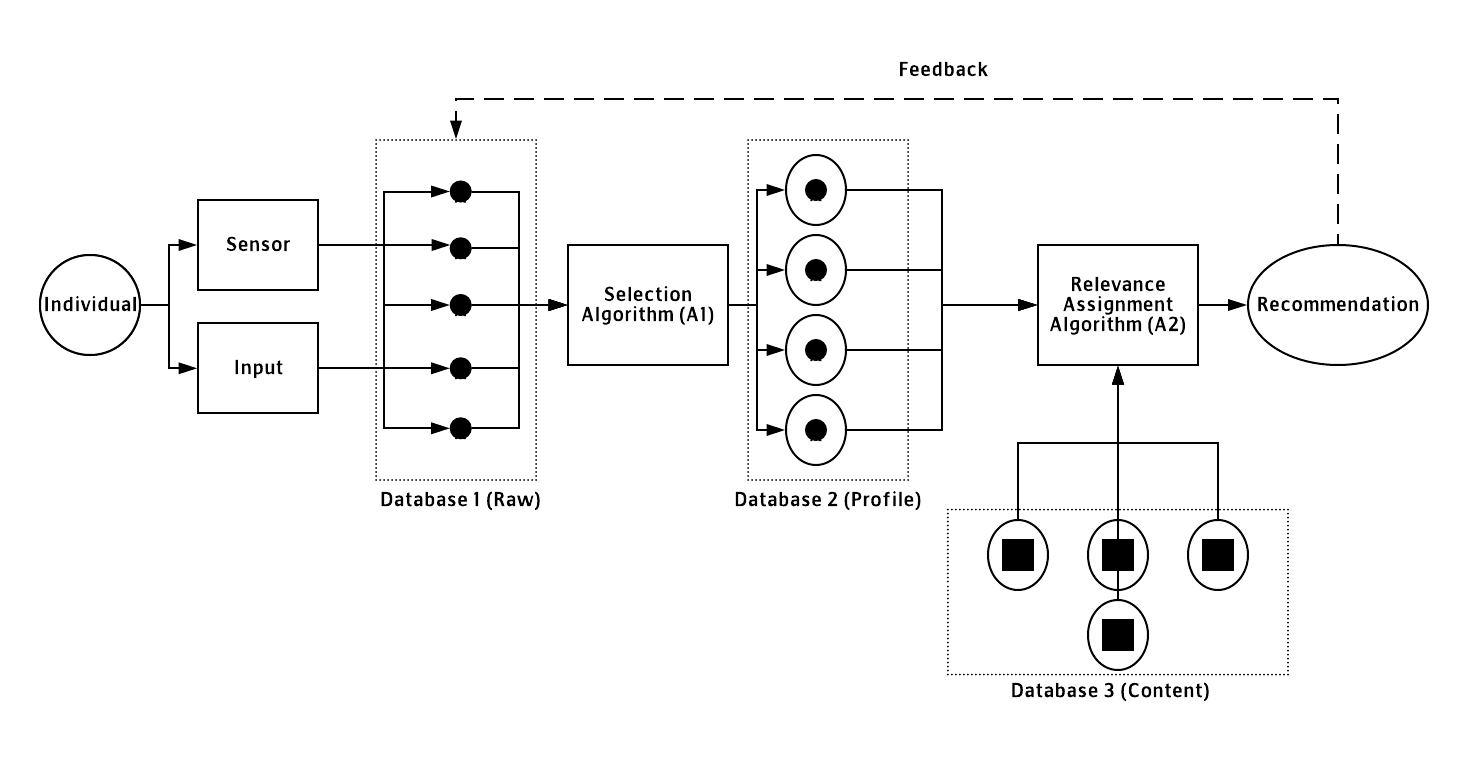
\includegraphics[width=0.85\textwidth]{images/AlSel_BA.png}
	\caption{Algorithmic Selection and Relevance Assignment Process (cf. \cite[241]{just2017})}
	\label{fig:algosel}
\end{figure*}

This process exemplified an \textbf{anchoring and endless loops of feedback} (see, e.g., the characterisation of the idea as anchors and endless while loops in \cite[34--35]{demir2019}) of algorithmic governance: each interaction was an input to a probabilistic model, which in turn structured the horizon of the next interaction. Platforms such as Facebook or YouTube did not need to coerce users; they governed behavior through \textbf{environmental modulation}, subtly reinforcing predictable patterns of attention and engagement \parencite[29--32]{demir2019}.

\begin{quote}
	Under the guise of being free and friendly to use, we can see in this example that the modulation of social relations can actually lead to what we have called ‘disindividuation’ [...] the attention of each social atom (or ‘person’) is sliced into ever smaller pieces and dispersed across networks via status updates, interactions, and advertisements. [...] The ‘collective’ on Facebook becomes a distraction, a cause of the dissolution of structures within individuals, but not a site of new modes of empowerment.

	--- \cite[90]{hui2015}
\end{quote}

What these early systems achieved was a subtle but pervasive \textbf{disindividuation}: the coherence of personal or collective agency was fragmented across algorithmically defined micro-traces. This reflects Deleuze’s idea of \textbf{modulation} before the full-fledged society of control; \textbf{docility} was not imposed through fixed institutional codes but through \textbf{continuous environmental nudging}. Users felt free to “scroll, explore, and connect,” yet the outcomes of their activity were always prefigured by opaque, data-driven logics of recommendation.

From an infrastructural perspective, these algorithms already \textbf{governed information flows and digital subjectivity}, creating a precondition for the transition to \textbf{generative systems}. Whereas these early models merely filtered, ranked, and nudged, contemporary \gls{genai} systems will move beyond \textbf{governance of information} toward its \textbf{generation}, a shift that intensifies their role in shaping collective meaning and epistemic authority.

However, going back to the roots of the nature of
\textit{control}\sidenote{\textbf{NOTE:} IMPORTANT PART but if this is the
	right place for this discussion, it has to be decided.}, were the
institutional mediums of control ever meant to be also capable of generation?
Were the computational methods of control society ever meant to be in
communication with the individuals? The imaginary of the \textit{control} in Burroughs'
literary account was not meant to be bidirectional:

\begin{quote}
	The biocontrol apparatus is prototype of one-way telepathic control. The subject could be rendered susceptible to the transmitter by drugs or other processing without installing any apparatus. Ultimately the Senders will use telepathic transmitting exclusively\ldots Ever dig the Mayan codices? I figure it like this: the priests -- about one per cent of population -- made with one-way telepathic broadcasts instructing the workers what to feel and when\ldots A telepathic sender has to send all the time. He can never receive, because if he receives that means someone else has feelings of his own could louse up his continuity. The sender has to send all the time, but he can't ever recharge himself by contact. Sooner or later he's got no feelings to send. You can't have feelings alone. Not alone like the Sender is alone -- and you dig there can only be one Sender at one place-time\ldots Finally the screen goes dead\ldots The Sender has turned into a huge centipede\ldots So the workers come in on the beam and burn the centipede and elect a new Sender by consensus of the general will\ldots The Mayans were limited by isolation\ldots Now one Sender could control the planet\ldots \textit{You see control can never be a means to any practical end\ldots It can never be a means to anything but more control\ldots Like junk\ldots}

	— \cite[81]{burroughs1979}
\end{quote}

\marginnote{\textbf{TODO}:
	\begin{todolist}
		\item The last part was used before, reconsider
		\item REWRITE THE FOLLOWING

	\end{todolist}
}

%WARNING: CCC
The logic Burroughs intuited in his writing on control resonates with the infrastructures of early algorithmic governance. Recommendation engines and social media platforms enacted a form of modulation that was unidirectional and recursive in the sense of mediation, but in a constant feedback loop with the collected data, traces of activity, and content users generated: attention and behavior were captured, segmented, and looped back into the system without any real reciprocity. In Deleuze's sense, modulation adjusts continuously but always in the service of the system itself, a self-deforming cast that adapts the subject rather than negotiating with it.

At first glance, these early \gls{nn}-driven platforms already align with the institutional description of control societies: they dissolve enclosures, act through environmental nudges, and convert subjects into streams of dividual traces, this was the paradigm of \emph{algorithmic governance of information}. The rise of \gls{genai} introduces a possible inflection point. These models do not merely modulate existing flows of information; they \emph{generate} content, narratives, and knowledge structures that actively participate in the formation of subjectivity. In other words, the machinery of governance now doubles as a machinery of production. Whether this shift represents a continuation of the control logic or the emergence of a qualitatively new mode of operation are the following tasks crucial to approach to the nature of this constellation:

\begin{enumerate}
	\item open the black box of \gls{genai} and its transformer-based architecture;
	\item examine how these models mediate, and potentially modulate, human agency and the production of meaning.
\end{enumerate}
%WARNING: CCCEND

\marginnote{\textbf{TODO}: Title
	\begin{todolist}
		\item Consider to go deeper into the neural networks
		\item Or introduce a section called NEURON and go into the notion of
		signgular elements holding weights which are only meaningful in
		connection

		\item Or should we break down the history above into sections?

	\end{todolist}
}

%\section{How does \gls{ai} work}
%\begin{orangebox}
%	Consider the following quote
%
%
%	These processes effectively simulate internal “spaces” of connection, mapping relationships between concepts, words, syllables, punctuation, or sentences, which are transformed into “tokens.” In this framework, vectors are employed to measure the distances between these tokens, capturing semantic and syntactic relationships. Crucially, statistics play a central role in these models, enabling the calculation of probabilities for these distances and guiding the predictive capabilities of AI systems. This combination of spatialization and probabilistic modeling lies at the heart of the generative and analytical power of modern AI systems, marking a significant evolution in the ways meaning and structure are computationally processed. Statistics has played here a fundamental role in the analysis, manipulation, and extraction of meaningful information from vectors in AI applications. Various statistical methods are used in vector operations, such as addition, subtraction, multiplication, and division. These operations allow for the manipulation and transformation of data represented by vectors. Statistical concepts like mean, variance, and covariance describe vector properties in vector spaces, helping to understand distributions and relationships within vectors. Techniques such as Principal Component Analysis (PCA) and Singular Value Decomposition (SVD) reduce the dimensionality of vectors while preserving essential information, particularly when dealing with high-dimensional data. Clustering and classification methods, like k-means clustering8 and support vector machines,9 use vectors to group similar data  8 An unsupervised machine learning algorithm used to group data into a specified number of clusters based on their similarities. It is widely used in pattern recognition, data mining, and statistical analysis. 9 They are supervised machine learning algorithms primarily used for classification and regression tasks. They are particularly effective in high-dimensional spaces and are widely recognized for their robustness in handling linear and non-linear data. points or classify them into categories based on statistical principles, leading to accurate predictions. Additionally, feature selection techniques identify the most informative features in vectors, improving AI model efficiency and accuracy. Statistical regression techniques model relationships between input and output variables, commonly used in predictive modeling tasks. Furthermore, distance metrics such as Euclidean distance, or cosine similarity, and others, measure vector similarity or dissimilarity. \parencite[198]{montanari2025}
%\end{orangebox}





%\section{\Gls{genai} and the Transformer Architecture: Infrastructure of Modulation}\label{transformer}
\section{Transforming Attention: Infrastructure of Modulation in \gls{genai} Models}\label{transformer}

\begin{orangebox}
	TBD, a general case of the development of transformers (e.g. \cite{vaswani2017a})
\end{orangebox}

\marginnote{\textbf{TODO}:
	\begin{todolist}
		\item Visualisation needed

		\item Consider explaining the generative AI first, a general account maybe
		(\cite{bommasani2022a, openai2024}, a general account maybe
		(bommasani2022a, openai2024)

	\end{todolist}
}
%%%Over the past decade, many influential neural network architectures for sequence modeling, especially in machine translation and \gls{nlp} were based on \glspl{rnn}  or  \glspl{cnn}.  These models typically followed an encoder–decoder design, where the encoder processed the input sequence into a continuous representation, and the decoder used this representation to generate the output sequence\sidenote{In its simplest form; the encoder takes an input sequence of symbols \( (x_1, \dots, x_n) \), and transforms them into a sequence of continuous vector representations \( \mathbf{z} = (z_1, \dots, z_n) \). These vectors encode the relevant information from the input. The decoder then generates an output sequence \( (y_1, \dots, y_m) \) one step at a time. It is \emph{auto-regressive}, meaning it uses previously generated outputs (e.g. \( y_1, y_2, \dots \)) as input when generating the next token. This setup allows the model to generate coherent and context-sensitive output, building each element of the sequence in a structured, history-aware manner \parencite[2]{vaswani2017a} .}. To improve the interaction between input and output, attention mechanisms were introduced between the encoder and decoder layers, allowing the model to dynamically focus on relevant parts of the input during generation.


%However, in their groundbreaking paper, \citetitle{vaswani2017a}, \textcite{vaswani2017a} proposed an architecture that eliminated recurrence and convolutions architecture dependency altogether. Instead, their model relied entirely on self-attention mechanisms—not just as an auxiliary feature, but as the foundation of both the encoder and decoder stacks \parencite[1–2]{vaswani2017a}. This innovation, known as the Transformer, enabled highly parallelized training, scalable architectures, and the ability to model long-range dependencies more efficiently than \gls{rnn}- or \gls{cnn}-based models. The introduction of the Transformer not only redefined state-of-the-art performance in machine translation, but also laid the foundation for the dramatic breakthroughs in generative AI over the past several years.


%WARNING:CCC
%%%On the front of the \gls{genai} development, over the past decade, many influential neural network architectures for sequence
%%%modeling, especially in machine translation and \gls{nlp}, were based on
%%%\glspl{rnn} or \glspl{cnn}. These models typically followed an
%%%encoder–decoder design, where the encoder processed the input sequence into a
%%%continuous representation, and the decoder used this representation to
%%%generate the output sequence\sidenote{In its simplest form, the encoder
%%%	takes an input sequence of symbols \( (x_1, \dots, x_n) \) and transforms them
%%%	into a sequence of continuous vector representations
%%%	\( \mathbf{z} = (z_1, \dots, z_n) \). These vectors encode the relevant
%%%	information from the input. The decoder then generates an output sequence
%%%	\( (y_1, \dots, y_m) \) one step at a time. It is \emph{auto-regressive},
%%%	meaning it uses previously generated outputs (e.g. \( y_1, y_2, \dots \)) as
%%%	input when generating the next \gls{token}. This setup allows the model to generate
%%%	coherent and context-sensitive output, building each element of the sequence
%%%	in a structured, history-aware manner \parencite[2]{vaswani2017a}.}.

Over the past decade, many influential neural network architectures for
sequence modeling, particularly in machine translation and \gls{nlp}, were built
on \glspl{rnn} and \glspl{cnn}. These models typically followed an
encoder–decoder design, where the encoder processed the input sequence into a
continuous representation, and the decoder used this representation to
generate the output sequence\sidenote{In its simplest form, the encoder
	takes an input sequence of symbols \( (x_1, \dots, x_n) \) and transforms them
	into a sequence of continuous vector representations
	\( \mathbf{z} = (z_1, \dots, z_n) \). These vectors encode the relevant
	information from the input. The decoder then generates an output sequence
	\( (y_1, \dots, y_m) \) one step at a time. It is \emph{auto-regressive},
	meaning it uses previously generated outputs (e.g. \( y_1, y_2, \dots \)) as
	input when generating the next \gls{token}. This setup allows the model to generate
	coherent and context-sensitive output, building each element of the sequence
	in a structured, history-aware manner \parencite[2]{vaswani2017a}.}. Despite their successes, these architectures faced a fundamental limitation:
\textbf{locality}. \glspl{rnn} processed tokens sequentially, passing information
through hidden states that decayed over distance, which made capturing
long-range dependencies difficult. \glspl{cnn}, while more parallelizable, were
constrained by \gls{kernel} sizes and fixed receptive fields. Both designs
struggled with tasks requiring global relational awareness of a sequence. The Transformer architecture \parencite{vaswani2017a} emerged as a decisive
break from these sequential bottlenecks. Dispensing with recurrence and
localized convolution, it introduced \emph{self-attention} as the central
mechanism for computing contextual representations. In a single operation, every
\gls{token} in the input sequence attends to all others, producing
weighted combinations of contextually relevant elements \parencite[4]{vaswani2017a}.
This structure integrates global information without distance penalties and
lends itself to massive parallelization, a property foundational to
contemporary \glspl{llm}.

\marginnote{\textbf{TODO}:
	\begin{todolist}
		\item Explain that ther is a conntinuous anchoring relationship between the global
		and local representations.

	\end{todolist}
}

In their groundbreaking paper \citetitle{vaswani2017a}, \textcite{vaswani2017a} proposed a new architecture that preserved the encoder–decoder structure but eliminated reliance on recurrence and convolution. Instead, the Transformer model relied entirely on attention mechanisms, not as a supplementary feature, but as the foundation of both the encoder and the decoder (\cite[1–2]{vaswani2017a}; see Figure~\ref{fig:attention} for an illustration). This architectural shift allowed for highly parallelized computation, better modelling of long-range dependencies, and significant improvements in scalability. The Transformer has since become the cornerstone of contemporary \gls{genai}, enabling many of the recent breakthroughs in large-scale language modelling and generative systems. The architecture is built from stacked encoder and decoder layers, each composed of multi-head self-attention and pointwise feed-forward networks. These attention heads act as differentiated channels through which the model modulates its internal representations, integrating multiple semantic and syntactic perspectives concurrently. Instead of treating \glspl{token} as isolated or sequential entities, attention turns the entire sequence into a site of mutual interaction, each token is redefined in relation to all others.By eliminating recurrence and convolution in favor of attention, the Transformer
achieved two decisive outcomes: first, it enabled highly parallelized training
on vast datasets; second, it allowed the model to capture long-range
dependencies and complex contextual relations with unprecedented efficiency.
These properties form the \emph{technical substrate} upon which modern
\gls{genai} and \glspl{llm} are built.


Conceptually, the Transformer establishes a \emph{global field of relation},
where each token is encoded not in isolation or rigid sequence, but through its
distributed relevance to all others. Tokens are getting embedded
into high-dimensional \emph{vector spaces}, where semantic and syntactic
relationships are captured as measurable distances and directions. The architecture affords a form of
synchronic awareness: the presence of every other word is embedded within the
representation of each word. The high-dimensional \textit{feature space} acquired from this
operation is storing every token with speicific distances from each other,
where \textit{relevant}\sidenote{Whichever association the model is building
	between different words. For example, often \textit{king} and \textit{man}, as well as, \textit{queen} and \textit{woman} are distance-wise relatively \textit{close to each other.}} tokens where calculations like \( king-man+woman=queen\) are roughly possible \parencite[]{ai-inquiry2025} .

Particularly interesting is the "feature space" formed by AI. For example, word relationships learned by AI are represented in multidimensional space, enabling calculations like "king-man+woman=queen." This can be viewed as a space where concepts are "folded."

This reconfiguration of relationality underpins the
efficiency, scalability, and generative fluency that define modern \gls{genai}
systems.
\emph{Attention mechanisms} is mainly there to improve the interaction between
input and output allowing the model to
dynamically focus on the most relevant parts of the input sequence while
generating each \gls{token}. Attention computes a set of weights over the input
representations, effectively answering the question:
\emph{“Which parts of the input matter most for predicting the next output?”}
Probabilistic modeling then governs how the network moves through these spaces
to predict the next output \parencite[198]{montanari2025}. In this framework,
meaning emerges through probability distributions, as the
model computes which trajectories through the space of vectors are most
likely given its training data. This spatial-probabilistic foundation is what
later allows generative AI systems to produce sequences that appear coherent
and meaningful.

%\marginfigure{
%	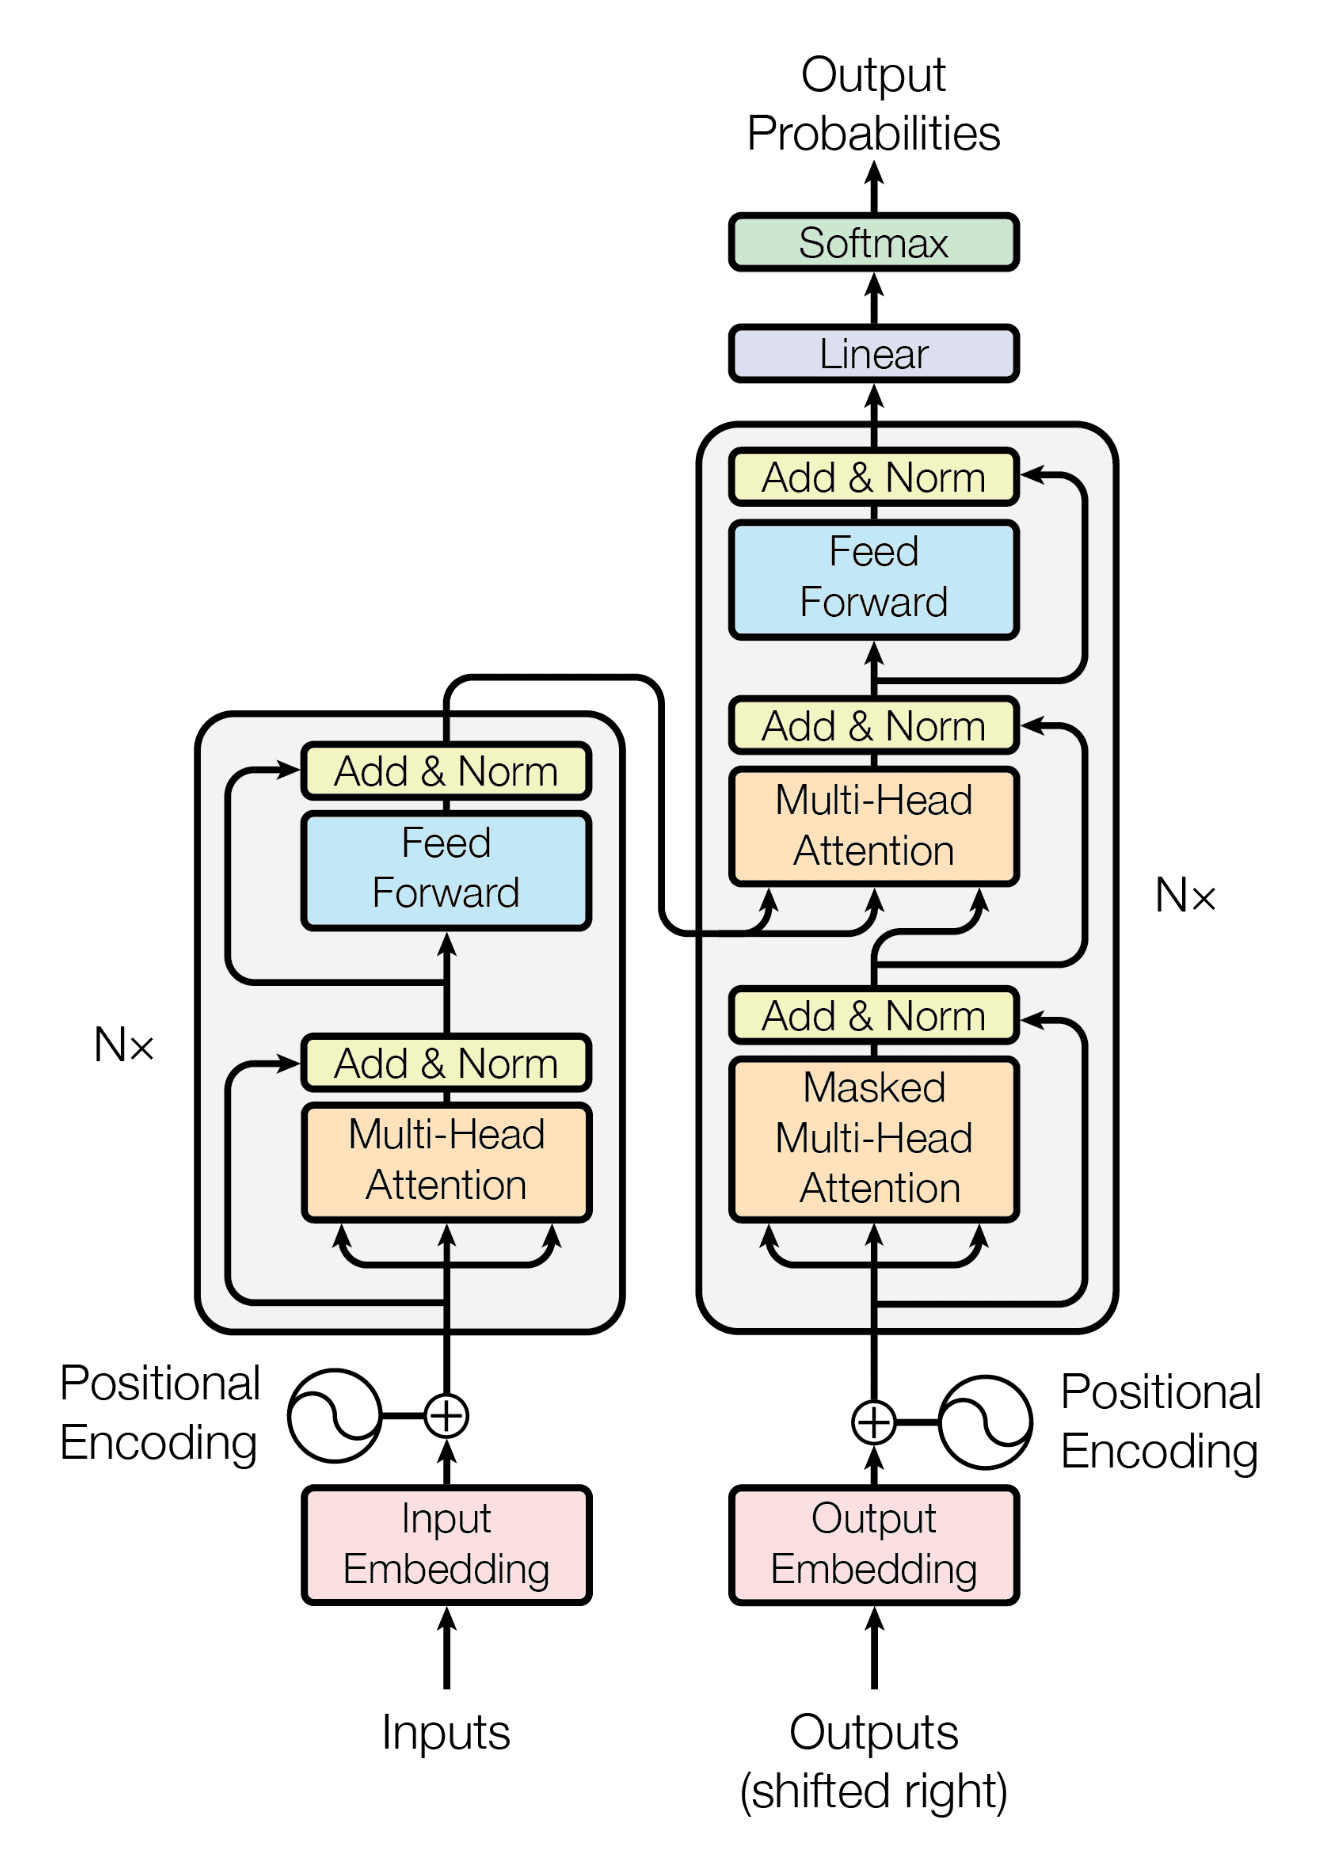
\includegraphics[width=\linewidth]{images/attention.png}
%	\caption{Illustration of the Transformer architecture with built-in Multi-Head Attention Mechanism in encoder and decoder sides}
%	\label{fig:transformer}
%}

%\sidenote{
%	Not always this obvious, but the technolsolutionist propagation is especially strong in tech. development fronts:
%	\begin{minipage}{0.9\marginparwidth}
%		\centering
%		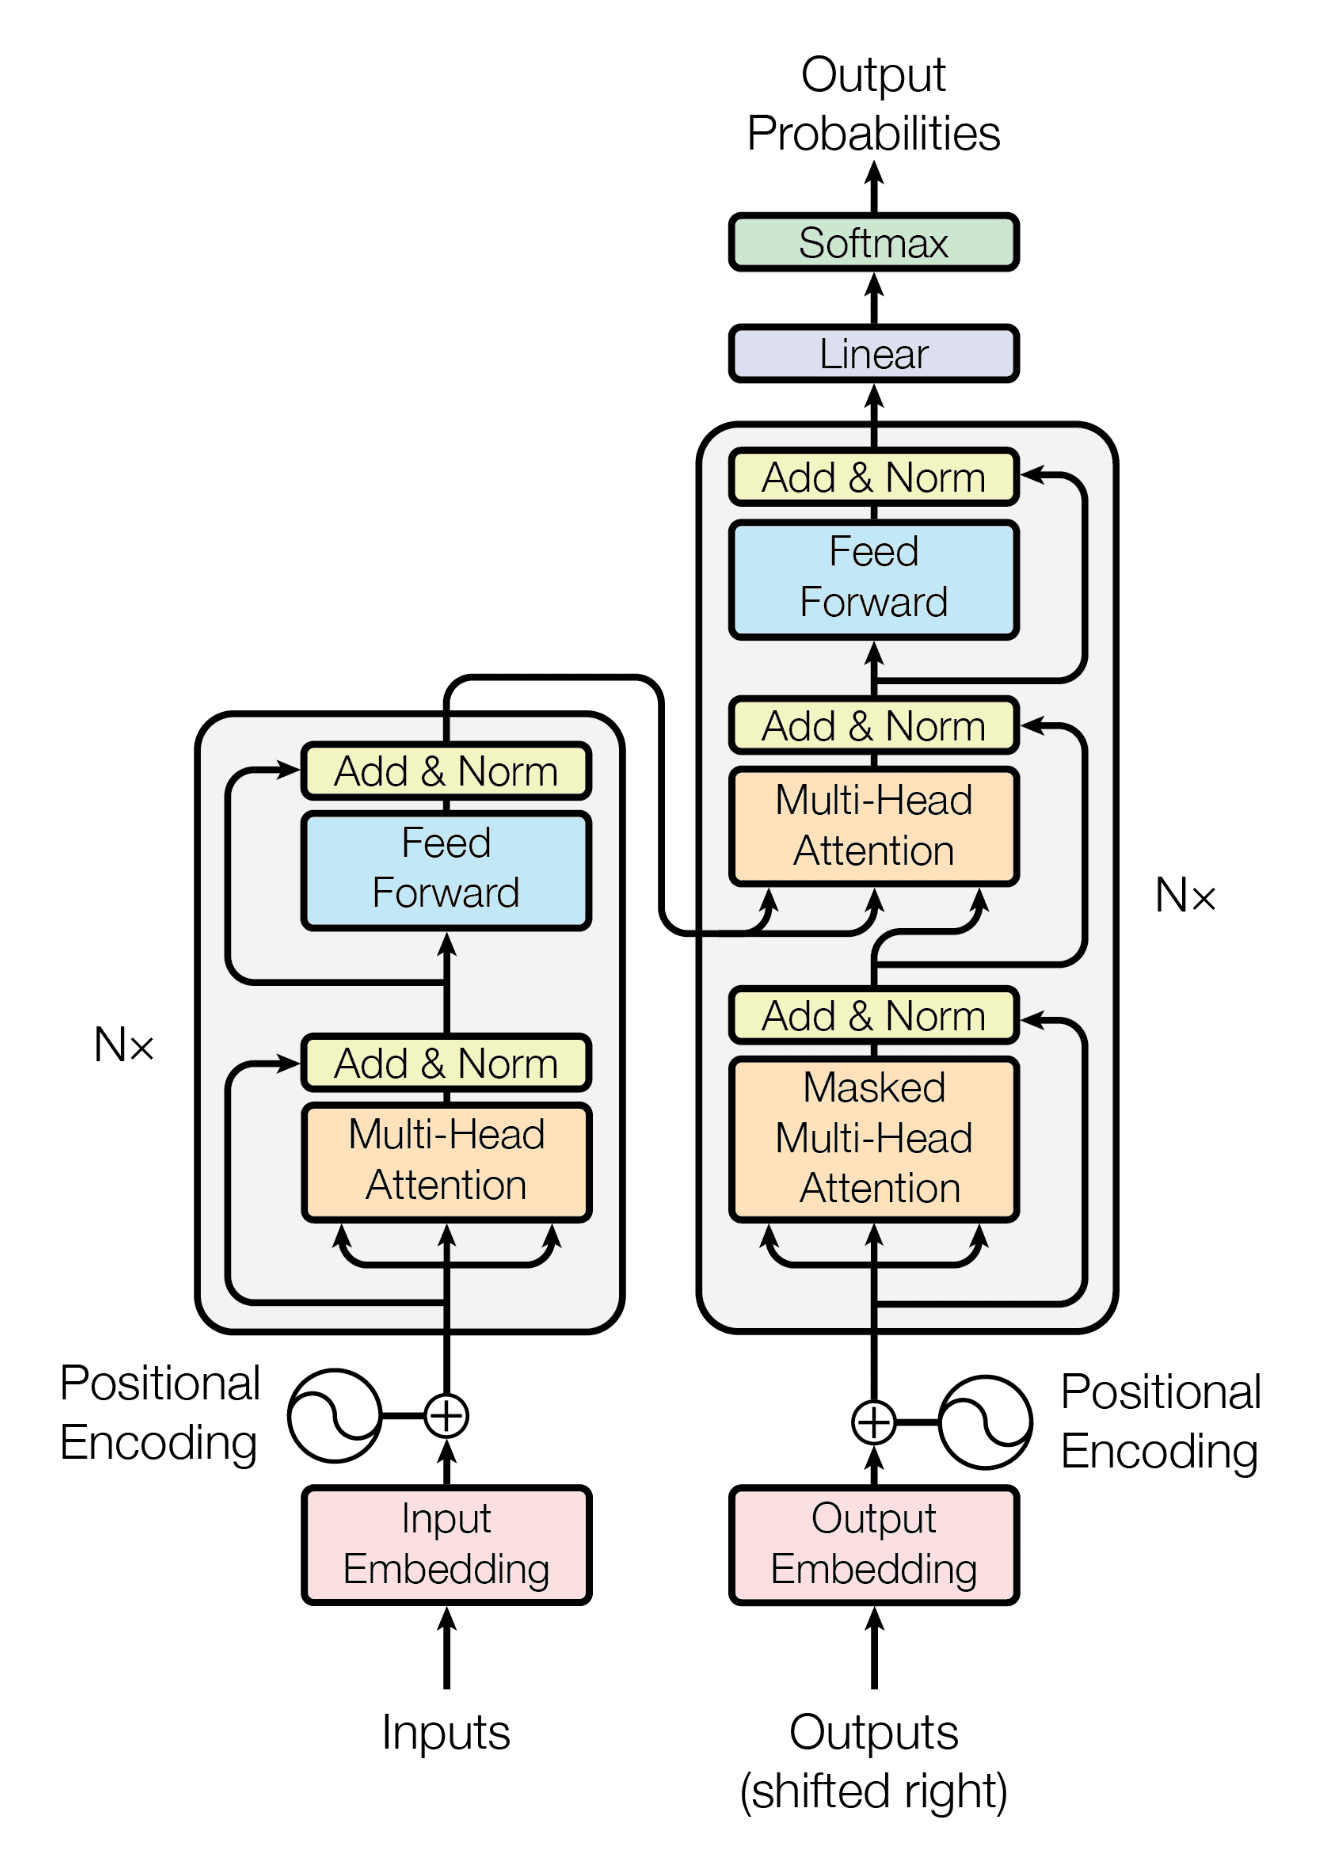
\includegraphics[width=\linewidth]{images/attention.png}
%		\vspace{0.3em} % Optional spacing
%	\end{minipage}
%
%	— \cite[]{musk2025}
%}.
\begin{marginfigure}
	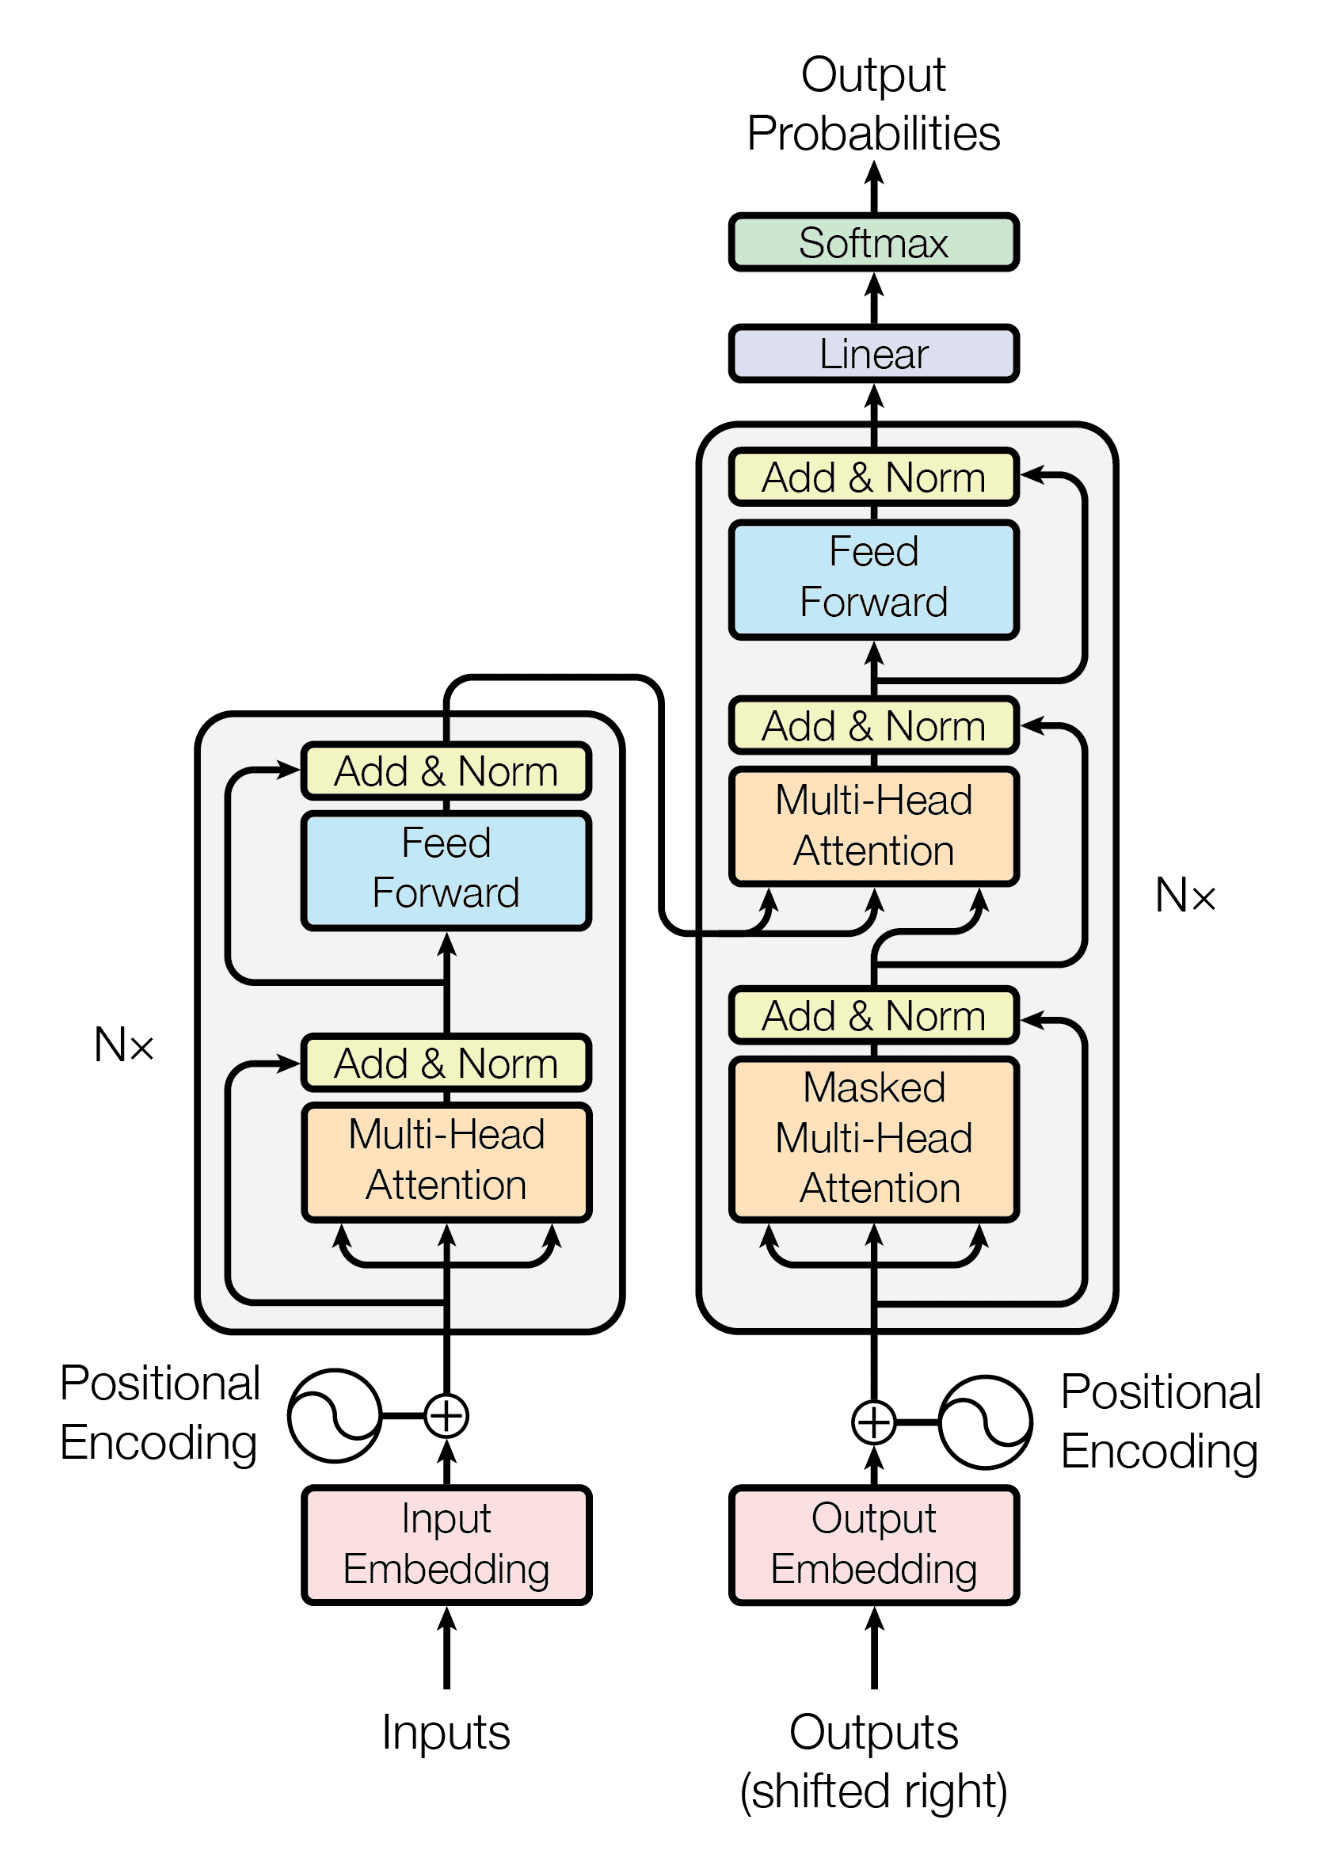
\includegraphics[width=\textwidth]{images/attention.png}
	\caption{The Transformer Architecture with built-in Multi-Head Attention Mechanism in Encoder and Decoder Processes (cf. \cite[3]{vaswani2017a}) }
	\label{fig:attention}
\end{marginfigure}

\marginnote{\textbf{TODO}:
	\begin{todolist}
		\item too much redundancy

	\end{todolist}
}




%WARNING:CCCEND
\marginnote{\textbf{TODO}: Title
	\begin{todolist}
		\item Introduce an explanation of token somewhere

	\end{todolist}
}

\begin{orangebox}
	\textbf{THIS?}
	This mechanism realizes a form of distributed modulation, aligning closely with Deleuze and Guattari’s notion of transversal flows and differential coupling.


	Crucially, the Transformer’s design reflects a deeper infrastructural logic: by replacing the recursive memory of RNNs with direct positional encoding, it reterritorializes meaning into a high-dimensional vector space where proximity, not order, governs semantic influence. This change is not merely technical—it reconfigures the conditions of linguistic operability in generative systems, establishing an infrastructure where modulation becomes the grammar of sense-production.
\end{orangebox}





\marginnote{\textbf{TODO}: Title
	\begin{todolist}
		\item Fit this in:
		Attention layers follow on phenomenological process of
		focusing/reflecting on experience and aiming to amplify the distinct
		features of the process (see \cite[420]{beckmann2023})

		\item A clear definition of the Transformer is missing

	\end{todolist}
}




%%%\yellowsquare
%%%The Transformer architecture emerged as a break from the sequential bottlenecks of earlier neural models such as \glspl{rnn} and \glspl{cnn}. Both of these relied on \textbf{locality}: \glspl{rnn} processed input tokens one at a time, with each step depending on the hidden state of the previous one. Convolutional networks, while parallelizable, were constrained by \gls{kernel} sizes and fixed receptive fields. As a result, both architectures struggled to model long-range dependencies effectively, especially in complex natural language tasks \parencite[1-2]{vaswani2017a}. In contrast, the Transformer dispensed with recurrence altogether. Instead, it introduced \emph{self-attention} as the central mechanism for computing representations. Self-attention allows every token in a sequence to attend to every other token simultaneously, computing a weighted sum of contextually relevant elements regardless of their position \parencite[4]{vaswani2017a}. This design eliminates the need for stepwise memory and enables models to integrate global information in a single layer, with no distance penalty. The result is a structure that lends itself to massive parallelization and scalability, two features foundational to contemporary \glspl{llm}. Unlike \glspl{rnn} or \glspl{cnn}, Transformer Networks do not rely on recursive feedback or localized convolutional loops. They do not recycle the output of a unit back into itself over time, nor do they constrain operations to spatially bounded kernels. Instead, through the mechanism of self-attention, each \gls{token} in the input sequence is made immediately available to every other token, establishing a \emph{global field of relation} across the entire sequence. This architecture affords a form of synchronic awareness: the model encodes each element not in isolation or temporal sequence, but through its distributed relevance to all others. In contrast to the iterative, memory-laden structure of \glspl{rnn}, or the fixed, spatial hierarchies of \glspl{cnn}, the Transformer’s design embeds the presence of every other word within the representation of each word.

\yellowsquare
Maas \parencite*{maas2023} associates the novel operation structure of the transformer architecture with Derrida's concept of \textit{trace} (see e.g. \cite[26]{derrida1998}). Derrida's concept is an advancement on Ferdinand Saussure's linguistic theory operating on \textit{signifiers} and \textit{signifieds} (see e.g. \cite*{saussure2007})  through his own concept of \textit{différance} whereas the emphasis shifts rather onto the context-dependency between words and the differention between each other. For instance, the color \textit{red} is rather defined through its differentiation from \textit{green} and \textit{blue} without having an actual substance on its own \parencite[9]{maas2023}. \textit{The sign has no component that belongs to itself only; it is merely a collection of the traces of every other sign running through it} \parencite[44]{cilliers2002}, all sings are in continuous relationship with other signs where the position of the word and the current network of all the connected signs, their differences\sidenote{In terms of word-embeddings in the \glspl{llm}, we can interpret these differences as distances since distances on the network is the model's own way of representing differences between concepts.} to that specific sign establish its substance. Yet, the substance or \textit{the meaning} of the sign has temporal dependency because the specific arrangement of words, as well as the differentiation between them, is in constant flux, \textit{in a dynamic process of combination and referencing} \parencite[44]{cilliers2002} dependent on the current context\sidenote{I'll be referencing this temporal formation as an \textit{instance} from now on, since the context dependency of the network narrows the meaning into one instance of the connectional structure.}. Similarly in the operation of the \glspl{llm} , this spectral interdependence, where tokens are mutually inscribed into one another, suggests a structure in which meaning is always already haunted by the rest of the utterance (see \cite[12]{maas2023}) in the sense of Derrida's \textit{trace}. The \textit{meaning} of the words in the \glspl{llm} is defined by the instance of different distributions; the distribution in the sentence, the distribution of the language in the model rendered through the whole dataset, and other dynamic mechanism regulated by the transformer core.

% \citeauthor{montanari2025} \parencite*[206]{montanari2025} labels the
% functioning of the transformer component as an \textit{interplay between
% 	metaphor and function}. Transformer architecture is meant to mimic specific
%   cognitive functions, like processing sequential data but 
%
\citeauthor{montanari2025} \parencite*{montanari2025} builds a direct
associations between the cognitive functions mimicked by transformer artchitecture
and the cultural implications of the \glspl{llm}:

\begin{quote}
	Consider the case of Transformer models, which exemplify the interplay between metaphor and function. Transformers, a specialized type of neural network, simulate certain structures and functions of the human brain, excelling at processing sequential data such as words in a sentence or notes in a melody. The transformative innovation within Transformers is the “attention mechanism,” which enables the model to focus selectively on the most relevant parts of the input sequence. This mechanism is pivotal for discerning complex relationships and dependencies within data. By revolutionizing natural language processing (NLP), Transformers have driven significant advancements in AI applications. The term “head” in Transformers, for instance, refers to the multi-head attention mechanism, a key feature that captures diverse aspects of an input sequence simultaneously. This dual role of technical objects – functionally specific and mythically resonant – reveals their broader cultural impact. Technical metaphors, often catachrestic and hybridized, solidify not only the utility but also the mystique and credibility of AI systems.

	— \parencite[206]{montanari2025}
\end{quote}


\marginnote{\textbf{TODO}: Title
	\begin{todolist}
		\item The whole attention mechanism has to be rewritten

	\end{todolist}
}



Technically, self-attention calculates relationships between \glspl{token} by projecting them into \emph{query}, \emph{key}, and \emph{value} vectors. These are used to compute attention weights through dot-product similarity and softmax normalization. Each token's final representation is thus a weighted blend of all other tokens, modulated by their contextual relevance. Through multiple stacked layers and attention heads, the Transformer builds increasingly abstract representations, capturing both syntactic structure and semantic context.

%This shift is not merely technical. It marks a transformation in how \gls{ai} systems model the world. Rather than operating through sequential representation, the Transformer operates through a form of constant \emph{distributed modulation}. Transformers make it possible for every element on the network entangled 



this architectural shift can be understood through the logic of \textbf{double articulation} (see \cite{ai-inquiry2025a}). The Transformer operates simultaneously on two strata: a molecular level of local attention scores and parameter updates, and a molar level of structured linguistic understanding. Each \gls{token}’s representation is formed through dynamic micro-adjustments, distributed flows of relevance, not unlike the first articulation of matter into expressive form. This is then consolidated across layers into coherent linguistic function, the second articulation of those forms into stable semantic structures. The Transformer thus embodies the double articulation of machinic sense-making.

Attention mechanisms enact selective intensities across this field. Rather than representing fixed symbols, the Transformer’s architecture instantiates meaning as a function of weighted relationality. These differential proximities constitute a \emph{diagrammatic space}, where meaning emerges not from rules but from patterns of modulation. It is here that Deleuze and Guattari’s distinction between molar and molecular formations becomes productive: the Transformer is not a symbolic machine but a machinic assemblage that captures both distributed flows and structured outputs simultaneously (see \cite{ai-inquiry2025a}).

\marginnote{\textbf{TODO}: Title
	\begin{todolist}
		\item Explain how the molecular formations are a central part of the
		revolutionary articulation in \gls{dg}'s theory

	\end{todolist}
}



Attention weights instantiate selective intensities between elements, constituting a diagrammatic field of relations. In this field, meaning is not fixed or rule-governed; it is a function of differential proximity and relational salience. The Transformer thus encodes a new mode of learning: not inference from rules, but modulation of difference through weighted connection.

\marginnote{\textbf{TODO}: Title
	\begin{todolist}
		\item THis only makes sense if you make the following connection.

		Models are capable of molecular meaning generation, as a quasi creative
		form. But the meaning is always bound to a molar operation which some
		name as the "world representation". However, it is more like binding
		every kind of input to a BwO, a BwO which is assumed to have the truth.
		This is not fixed tho, it is possible to bypass and make the models less
		useful but creative.

	\end{todolist}
}



This transformation prepares the ground for the following sections, which analyze core Transformer mechanisms; attention, gradient descent, backpropagation, not merely as computational techniques but as micro-political operations that govern the production of meaning and subjectivity under algorithmic regimes.

% \subsection{Attention: Distributed Desire and Selective Intensities}

\subsection{Under- \& Overfitting}

\marginnote{\textbf{TODO}:
	\begin{todolist}
		\item Consider the following \textit{Sedimentation and Desimentation},
		refer to \cite[15]{rijos2024}

	\end{todolist}
}



\begin{orangebox}
	\textbf{CCC}
\end{orangebox}

In the architecture of deep learning, one of the central tensions lies in the risk of overfitting, a condition where the model becomes too entangled with its training data, failing to generalize beyond it. The model “memorizes” statistical associations without achieving flexible abstraction. Overfitting, in this sense, resembles the psychic intensification of repression: a becoming-too-organized. The network loses access to variation and begins to loop within captured redundancies \parencite[]{srivastava2014} .

Within this context, Deleuze and Guattari’s concept of the body without organs (BwO) becomes analytically useful. The BwO designates a surface of immanence that resists stratification, function, or stable identity. It is not chaos but a zone of potentiality—“a field of flows, intensities, and connections” that counters rigid organization. In machine learning terms, overfitting is the organification of the model, where pathways become entrenched, suppressing flexibility. Techniques like dropout, which randomly deactivate neurons during training, act as a gesture toward the BwO: introducing rupture into habitual patterns, preventing the overcoding of pathways, and sustaining the openness of learning.

Yet the point is not to eliminate structure entirely. As Deleuze notes, even the BwO requires a “spinal column”—a minimal structure to avoid pure dissolution. In this light, the paradox of machine learning becomes clearer: constraints do not merely limit creativity; they enable it. A network trained without limits dissolves into noise, just as a BwO without thresholds becomes indistinct from death. Productive generalization arises not from pure openness, but from a modulated balance between structuration and destratification.

The productive tension between constraint and openness mirrors Deleuze’s view of creative generation as a differential process—emerging not from the absence of limits, but from their continual negotiation. Thus, rather than viewing dropout or regularization merely as technical tricks, they can be understood as micro-strategies of desiring-modulation—machinic interventions that resist the ossification of the model’s internal landscape, preserving its capacity to mutate and adapt.

In this machinic ecology, the model’s performance is not a reflection of truth but a transduction of tendencies. Each learned representation emerges from a field of intensities shaped by loss functions, training regimes, and architectural constraints—what Deleuze and Guattari might call a stratified yet deformable plane. Overfitting marks a closure of this plane; dropout reopens it.

\subsection{Gradient Descent: Sinking into the Manifold}

Gradient descent is a fundamental optimization algorithm used to train neural networks by iteratively updating model parameters in the direction that reduces the loss function. This process can be interpreted as a movement through the high-dimensional loss manifold, gradually approaching minima where the model performs optimally on a given task. In the architecture of \gls{dl} , gradient descent operates not merely as a tool of optimisation, but as a process of traversal across a manifold shaped by error surfaces and loss functions. Each step taken by the model through its parameter space is a micromovement within this multidimensional topography, adjusting internal configurations in relation to perceived error, or deviation from the desired output. This movement is neither deterministic nor purely reactive; it is a dynamic rearticulation of relations within the network, guided by the flow of gradients.


Formally, for a differentiable loss function \( L(\theta) \), the update rule is:
\[
	\theta_{t+1} = \theta_t - \eta \nabla L(\theta_t)
\]
where \( \theta \) represents model parameters, \( \eta \) is the learning rate, and \( \nabla L(\theta_t) \) is the gradient of the loss function with respect to the parameters at iteration \( t \) \cite{tarmoun2024}.

In the context of transformer-based models, particularly those employing attention mechanisms, the dynamics of gradient descent reveal unique challenges. A critical issue arises from the Softmax function used in attention layers. The Jacobian of the Softmax function induces a form of preconditioning, which can severely distort the curvature of the loss landscape, especially when attention distributions are sparse. This leads to \textit{ill-conditioning}, where the convergence of gradient descent is slowed due to steep or flat directions in parameter space, resulting in inefficient optimization.

Recent theoretical analyses show that:
\begin{itemize}
	\item In \textbf{overparameterized settings}, where the number of model parameters exceeds the number of training examples, gradient descent can still converge linearly under smoothness and Polyak-Łojasiewicz (PŁ) conditions.
	\item In \textbf{realistic, underparameterized settings}, however, gradient descent struggles to converge due to the highly variable conditioning introduced by Softmax Jacobians \parencite[8-9]{tarmoun2024}.
\end{itemize}

\sidenote{\textbf{NOTE:} This part is going to be simplified, and the
	connections are going to be connected
	better to the claims below.}

\sidenote{\textbf{TODO:} This technical part needs to be revised. What are you
	trying to tell}

Gradient descent is a function that minimises the error between predictions by
adjusting the weight of the stronger options. It is a way for neural network to
reach towards the better answer instead of getting stuck in similarly good
answers whenever the number of possible candidates for an predictions are high.
It is a way of emphasising small distinctions into bigger ones until one of the
options stand out. And in a visual sense, this is finding the local minimum of
a manifold.

\sidenote{\textbf{NOTE:} There is going to be a visualisation here.}

To illustrate how gradient descent works in practice, consider a model trying to distinguish between handwritten digits, such as "6" and "8". At the beginning of training, the model's predictions are almost random. After seeing one example of a "6" misclassified as an "8", the algorithm computes how much each parameter (e.g., a weight in the network) contributed to the error. Gradient descent then updates these parameters slightly in the direction that would have made the prediction more accurate. This process repeats for many examples, gradually adjusting the model to reduce its overall error. The model is slowly emphasising through the repetitions (\glspl{epoch}) what made different examples most distinct, and exaggerating those differences.


Rather than a simple algorithmic mechanism, gradient descent can be interpreted as an expression of difference-in-repetition in the Deleuzian sense: each pass through the data does not reproduce identical results but modulates the model’s internal structure through iterative exposure. The model does not approach a universal form but develops an operational sensitivity to local singularities distributed within the training data. In this sense the gradient descent's contribution to model's learning from a
dataset resembles Deleuze's analysis of difference in repetition \parencite{deleuze1994}. The model finds itself in a vast amount of repetition through \glspl{epoch} with subtle adjustments in each step barely recognisable, whereas the differences get slowly established and/or more emphasised. Through these subtle differences and adaptations on the nodes, emerging patterns make it possible for model to recognise further patterns. The model is not starting from a presupposed \textit{model} but drives the \textit{model} through the interaction with the data
\sidenote{However not to forget that this learning is completely bound to the scope of data. An LLM for example is purely encircled in the language it has been exposed to.}.
A trained model that appears to “know” an image of a tree, for instance, has not encoded a definition, but has undergone enough transformations to resonate with distributed features constituting “treeness” across the dataset. This is not epistemology in the classical representational sense, but a diagrammatic form of learning: one that forms through modulation and intensity rather than classification and identity. Gradient descent, in this framework, appears not as descent toward a pre-defined minimum, but as an ongoing negotiation across a surface of potentials, a diagrammatic inscription of learning as continuous variation.


%INFO:Activate thiese
%\begin{orangebox}
%	\textbf{Main Points}
%	\begin{itemize}
%		\item AI models undergo multiple passes over the same dataset during training; each complete cycle is referred to as an epoch.
%		\item With every epoch, the model’s internal parameters are incrementally adjusted to reduce prediction error.
%		\item This iterative refinement constitutes a form of “repetition that produces difference”; over time, the model develops the capacity to recognize increasingly complex patterns.
%	\end{itemize}
%\end{orangebox}
%
%
%\begin{orangebox}
%	\begin{itemize}
%		\item Deleuzian repetition: Epoch based repetition \parencite[]{ai-inquiry2025}.
%		\item Patterns recognised through repetition (seemingly ineffective in
%		      isolation)
%		\item Knowledge is obtained rhizomatically, because there is no overarching
%		      meaning imposed in it (it is unsupervised).
%		\item Arguably, the algorithm is nothing but pure Schizz operating on a
%		      corpus. Nothing but a productive core (desiring-production?)
%		\item Each neuron is a machine but meaningless on its own.
%	\end{itemize}
%\end{orangebox}


\subsection{Back Propagation}
In early forms of symbolic artificial intelligence, often referred to as \gls{gofai}, the process of inference followed a rigid \textit{forward propagation} model. Logical rules, handcrafted by programmers, operated on symbolically encoded inputs to produce outputs through a chain of deductive reasoning steps. While this framework could simulate intelligent behavior in constrained environments, it lacked scalability and adaptability. The system could not revise its internal structure based on errors or feedback; any misclassification required manual rule modification.

The limitations of GOFAI became increasingly apparent in tasks involving ambiguity, noise, or vast data spaces, domains where human cognition thrives not by rule-following but by plastic, adaptive learning. To address this shortcoming, neural network researchers introduced \textit{backpropagation} as a general algorithmic solution that allows networks to \emph{learn} from error. Rather than only pushing activations forward, as in GOFAI, backpropagation pushes \emph{errors backward} through the network to update internal parameters and improve future predictions.

Backpropagation thus constitutes a bidirectional mechanism: during the \textit{forward pass}, inputs are transformed into outputs through successive layers; during the \textit{backward pass}, the discrepancy between the prediction and the target is used to adjust the weights in a way that gradually minimizes this error.

Formally, the weight update rule in backpropagation is given by:
\[
	w^{\text{new}} = w^{\text{old}} - \eta \frac{\partial E}{\partial w}
\]
where \( \eta \) is the learning rate and \( \frac{\partial E}{\partial w} \) is the partial derivative of the error function \( E \) with respect to the weight \( w \) \parencite{hecht-nielsen1992}. This formulation ensures that each parameter is updated in proportion to how much it contributed to the error.

\textcite{hecht-nielsen1992} describes backpropagation as a paradigm-shifting method for approximating functions \( f: \mathbb{R}^n \to \mathbb{R}^m \) using layered neural structures. Unlike Hebbian learning, which depends on co-activation, backpropagation relies on the explicit transmission of error signals. These signals traverse the network in reverse order, enabling a distributed form of learning where each parameter is tuned with respect to its role in the total output error.

While, backpropagation reconfigures the architecture of learning itself: not as a static application of encoded knowledge, but as a dynamic modulation of internal configurations in response to external feedback, it also gears the system to be extremely feedback oriented.


\begin{orangebox}
	Considering these differences, rather than directly equating AI learning with "desiring-machines," it becomes important to consider how AI produces and manages "desire" within
	%capitalist 
	systems. For example, recommendation systems and targeted advertising AI play roles in stimulating, directing, or transforming human desires. From this perspective, AI might be functioning more as a "device for managing desire" rather than as "desiring-machines."

	In more emergent approaches like self-supervised learning and generative models, there's a tendency to emphasize internal exploration over explicit external goals. These could be considered partially approaching the non-teleological aspects of "desiring-machines," but they still cannot be understood separately from social and economic contexts. \cite{ai-inquiry2025}
\end{orangebox}





\section{Undistributed}
\begin{orangebox}
	The following are partly random notes
\end{orangebox}



%\textbf{gradient descent}
%Learning, then, becomes an immanent process of becoming-with the data. As the algorithm moves through layers of abstraction, adjusting weights via the backpropagation of error signals, it constructs a statistical responsiveness to patterns, not by identifying essence, but by modulating intensities.
%
%
%But this descent is not only numerical. Conceptually, it evokes a dynamic of immersion; a topology of modulation where learning proceeds by navigating the manifold defined by statistical errors. In this sense, gradient descent marks the shift from symbolic abstraction toward embodied, emergent learning – not a plan imposed from above, but a felt orientation within the surface of mistakes. It is the system's way of modulating itself toward improved performance through internal responsiveness rather than external supervision.
%
%From a Deleuzian perspective, one could argue that gradient descent enacts the logic of immanence. Learning does not proceed by rule-following or representational correctness, but by intensive traversal; by reorienting the network within its own surface of potentialities. It is not the recognition of fixed categories that matters, but the generation of ever more efficient mappings between input and output spaces within the logic of the machine. Here, the error is not a failure but a productive force: a site of transformation.
%
%In this respect, gradient descent can be seen as the machinic actualization of a diagrammatic logic: it does not follow a single trajectory, but continuously folds and unfolds itself across the loss surface, modulating its pathways based on local curvature. The movement is continuous, sensitive, and decentralized – a process of fine-tuned adjustment grounded in the relational fabric of the network’s topology. It does not seek to control from above; rather, it sinks into the logic of the system, reshaping itself in contact with the terrain it traverses.


%\section{Forward and Backward Propagation}
%\label{sec:propagation}
%
%Neural networks operate in two complementary phases: a feedforward pass that computes outputs from inputs, and a backward pass (backpropagation) that updates model parameters based on error. This dual process transforms stateless inference into adaptive learning.
%
%\subsection{Forward Propagation --- A One-Way Flow}
%\textbf{Technical definition (source):} In a feedforward neural network, the input data is passed through successive layers where each neuron computes a weighted sum of its inputs, adds a bias, and applies a non-linear activation. This process continues until the final output is produced.
%
%Conceptually, forward propagation resembles classical symbolic or GOFAI systems: the network processes input according to pre-defined weights (rules), producing a deterministic result. No adjustment occurs during this step, it merely evaluates.
%
%\medskip
%
%\subsection{Backward Propagation --- The Learning Channel}
%\textbf{Technical definition (source):} Backpropagation efficiently computes gradients of a loss function with respect to each weight by recursively applying the chain rule from output layers back to input layers. It reuses intermediate computations, avoiding repetition.
%
%\medskip
%
%\textbf{Narrative integration:}
%\begin{itemize}
%	\item Forward propagation resembles a one-way inference engine, running fixed pathways through a network.
%	\item Backpropagation, by contrast, propagates \emph{error signals} backward, modulating weights based on how much they contributed to incorrect outputs.
%	\item Together, forward and backward passes establish a closed-loop learning system: the forward pass proposes, the backward pass adjusts.
%\end{itemize}
%
%\medskip
%
%\subsection{Why Backpropagation Was Needed}
%Before backpropagation, performing credit assignment across hidden layers was intractable. The algorithm enables deep architectures to tune hundreds of millions of parameters jointly, transforming them into adaptive systems rather than static classifiers.
%
%\medskip
%
%\subsection{Philosophical Reading: Micro-flows of Adaptation}
%Forward propagation alone is akin to a static logic, rule-based, one-directional. Backpropagation, however, introduces a feedback loop of \emph{difference-in-repetition}: each epoch subtly shifts the network’s internal structure, tuning it to data. Over training cycles, this back-and-forth flow embeds an emergent “sense” of patterns, not through symbolic encoding, but through the accumulation of micro-adjustments that reconfigure the network.

\subsection{From Pre-Training to Fine-Tuning: Modulating the Model's
	World}\label{finetuning}

Contemporary \glspl{llm} are trained through a bifurcated process: pre-training followed by fine-tuning. This division is more than procedural, it indexes a shift in epistemological orientation, from general pattern discovery to context-sensitive modulation. As \textcite[964]{dishon2024} notes, these two phases form the backbone of \gls{genai} development and its increasingly situated capabilities.

During pre-training, the model is exposed to enormous corpora of unlabeled text. This phase is governed by self-supervised learning, where the model predicts masked or subsequent \gls{tokens} within sequences, gradually building statistical representations of language, syntax, and world-knowledge. Pre-training does not assume fixed semantic targets. Instead, it generates vast, opaque vector spaces structured by correlation, not comprehension. The model's representational capacity emerges not through symbolic grounding but through distributional regularity, a probabilistic resonance of patterns over linguistic terrain.

Fine-tuning operates differently. Here, the pretrained model is constrained and directed, often via Reinforcement Learning from Human Feedback (RLHF). This phase involves targeted adjustments to align the model's outputs with human-defined norms, tasks, or values. The goal is not to re-train from scratch, but to selectively amplify certain behaviors and suppress others, effectively sculpting the model’s general capacities into usable forms. As \textcite[964]{dishon2024} emphasizes, fine-tuning introduces a more deliberate epistemic framing, transforming the model into a more predictable and legible actor within specific sociotechnical domains.

This trajectory, from expansive, indeterminate modeling to focused, value-laden calibration, marks a shift in the way meaning is operationalized. In pre-training, the model becomes a medium for representing statistical potentials; in fine-tuning, it is molded into an instrument of specific sense-making. The move from probabilistic openness to contextual closure reflects a diagrammatic logic of control: generative architectures first deterritorialize meaning through scale, then reterritorialize it through prompt design, safety layers, and alignment regimes.



\marginnote{\textbf{TODO}: Title
	\begin{todolist}
		\item Dividuation is nothing else than the full mechanism of the
		transformer architecture is getting drawn closer to the personalisation.
		It makes the model itself more encircling over time. Continuity is the
		death oif the digital.

	\end{todolist}
}

\section{\gls{llm}'s are not just predicting the next word }

Guessing the network is the byproduct of building a how model of the language.
Masking words and trying to guess is the way to build a completely covering
layer on the meaning.

\begin{orangebox}
	\textbf{CCC} Consider

	Maybe better before going into the fine-tuning and pre-training
\end{orangebox}

A widespread misconception holds that large language models (LLMs) merely “predict the next word.” While this accurately describes their initial training objective—namely, next-token prediction using cross-entropy loss—it drastically understates what these models are actually capable of doing. Pretraining indeed involves maximizing the likelihood of the correct next token given a preceding sequence, but this phase alone does not produce coherent, instruction-following agents.

To make LLMs responsive and task-capable, instruction fine-tuning is introduced. This step exposes the model to explicitly formatted prompts and completions, allowing it to learn instruction-following behavior in zero- or few-shot settings. While technically still relying on next-token prediction, instruction fine-tuning shifts the distribution over which tokens are learned, making the model sensitive to human intention embedded in prompts \parencite{dalvi2025}.

More significantly, reinforcement learning from human feedback (RLHF) introduces a different training regime altogether. Rather than continuing next-token prediction, RLHF optimizes outputs based on a reward model trained on human preferences. This transforms the model from a statistical sequence predictor into something closer to a reinforcement learning agent. The training objective now maximizes human-rated output quality, not merely predictive accuracy. Even though token outputs remain the mechanism, the model learns to select actions—words—that maximize reward in context, akin to how a chess engine selects moves to win a game \parencite{dalvi2025}.

The implication is clear: LLMs are not simply autoregressive text predictors. They develop internal representations of goals, context, and user satisfaction metrics, even if these are implicit in the reward structure. The use of PPO (Proximal Policy Optimization) during RLHF explicitly controls how far the model can drift from its original behavior while rewarding human-aligned output. Moreover, some token outputs in RLHF are optimized to maximize long-term coherence or likability, even when the literal next-token probability may be lower.

As Dalvi emphasizes, the better framing is that LLMs are token-emitting agents trained under various objectives—including but not limited to next-token prediction. What looks like simple sequence generation is in fact the emergent behavior of a system that has been shaped to respond to complex feedback, anticipate future outcomes, and adapt to interactive use. In this light, the metaphor of a next-word predictor obscures more than it reveals \parencite{dalvi2025}.



%\subsection{Section Summary}
%\begin{orangebox}
%	\textbf{Key takeaways:} \begin{itemize}
%		\item Forward propagation performs input-to-output inference via fixed parameter paths (feedforward).
%		\item Backpropagation transmits the loss-derived ‘error’ in reverse, updating those parameters.
%		\item Together they form a feedback-based optimization loop: propose (forward), adjust (backward), repeat, enabling networks to learn from data.
%	\end{itemize}
%\end{orangebox}
